\part{Basic data structures in C\#}
\frame{\partpage}

\begin{frame}{Memory allocation}
	\begin{itemize}
		\pause\item Memory is allocated in \textbf{blocks}
		\pause\item The program specifies the size, in bytes, of the block it wants
		\pause\item The OS allocates a \textbf{contiguous} block of that size
		\pause\item The program owns that block until it frees it
		\pause\item Forgetting to free a block is called a \textbf{memory leak}
			(not really possible in Python, but a common bug in C++)
		\pause\item Blocks can be allocated and deallocated at will, but can \textbf{never grow or shrink}
	\end{itemize}
\end{frame}

\begin{frame}{Containers}
	\begin{itemize}
		\pause\item Memory management is hard and programmers are lazy
		\pause\item Containers are an \textbf{abstraction}
			\begin{itemize}
				\pause\item Hide the details of memory allocation, and allow the programmer to write simpler code
			\end{itemize}
		\pause\item Containers are an \textbf{encapsulation}
			\begin{itemize}
				\pause\item Bundle together the data's representation in memory along with the algorithms for accessing it
			\end{itemize}
	\end{itemize}
\end{frame}

\begin{frame}{Arrays}
	\begin{itemize}
		\pause\item An \textbf{array} is a contiguous block of memory in which objects are stored,
			equally spaced, one after the other
		\pause\item Each array element has an \textbf{index}, starting from zero
		\pause\item Given the address of the $0$th element, it is easy to find the $i$th element:
	\end{itemize}
	$$ \text{address}_i = \text{address}_0 + (i \times \text{elementSize}) $$
	\begin{itemize}
		\pause\item E.g.\ if the array starts at address $1000$ and each element is $4$ bytes,
			the 3rd element is at address $1000 + 4 \times 3 = 1012$
		\pause\item Accessing an array element is \textbf{constant time} $O(1)$
	\end{itemize}
\end{frame}

\begin{frame}{Lists}
	\begin{itemize}
		\pause\item An array is a block of memory, so its size is \textbf{fixed} once created
		\pause\item A \textbf{list} is a variable size array
		\pause\item When the list needs to change size, it \textbf{creates} a new array,
			\textbf{copies} the contents of the old array, and \textbf{deletes} the old array
		\pause\item Implementation details: \url{http://www.laurentluce.com/posts/python-list-implementation/}
	\end{itemize}
\end{frame}

\begin{frame}{Time taken to append an element to a list of size $n$}
	\begin{center}
		\vspace{-5ex}
		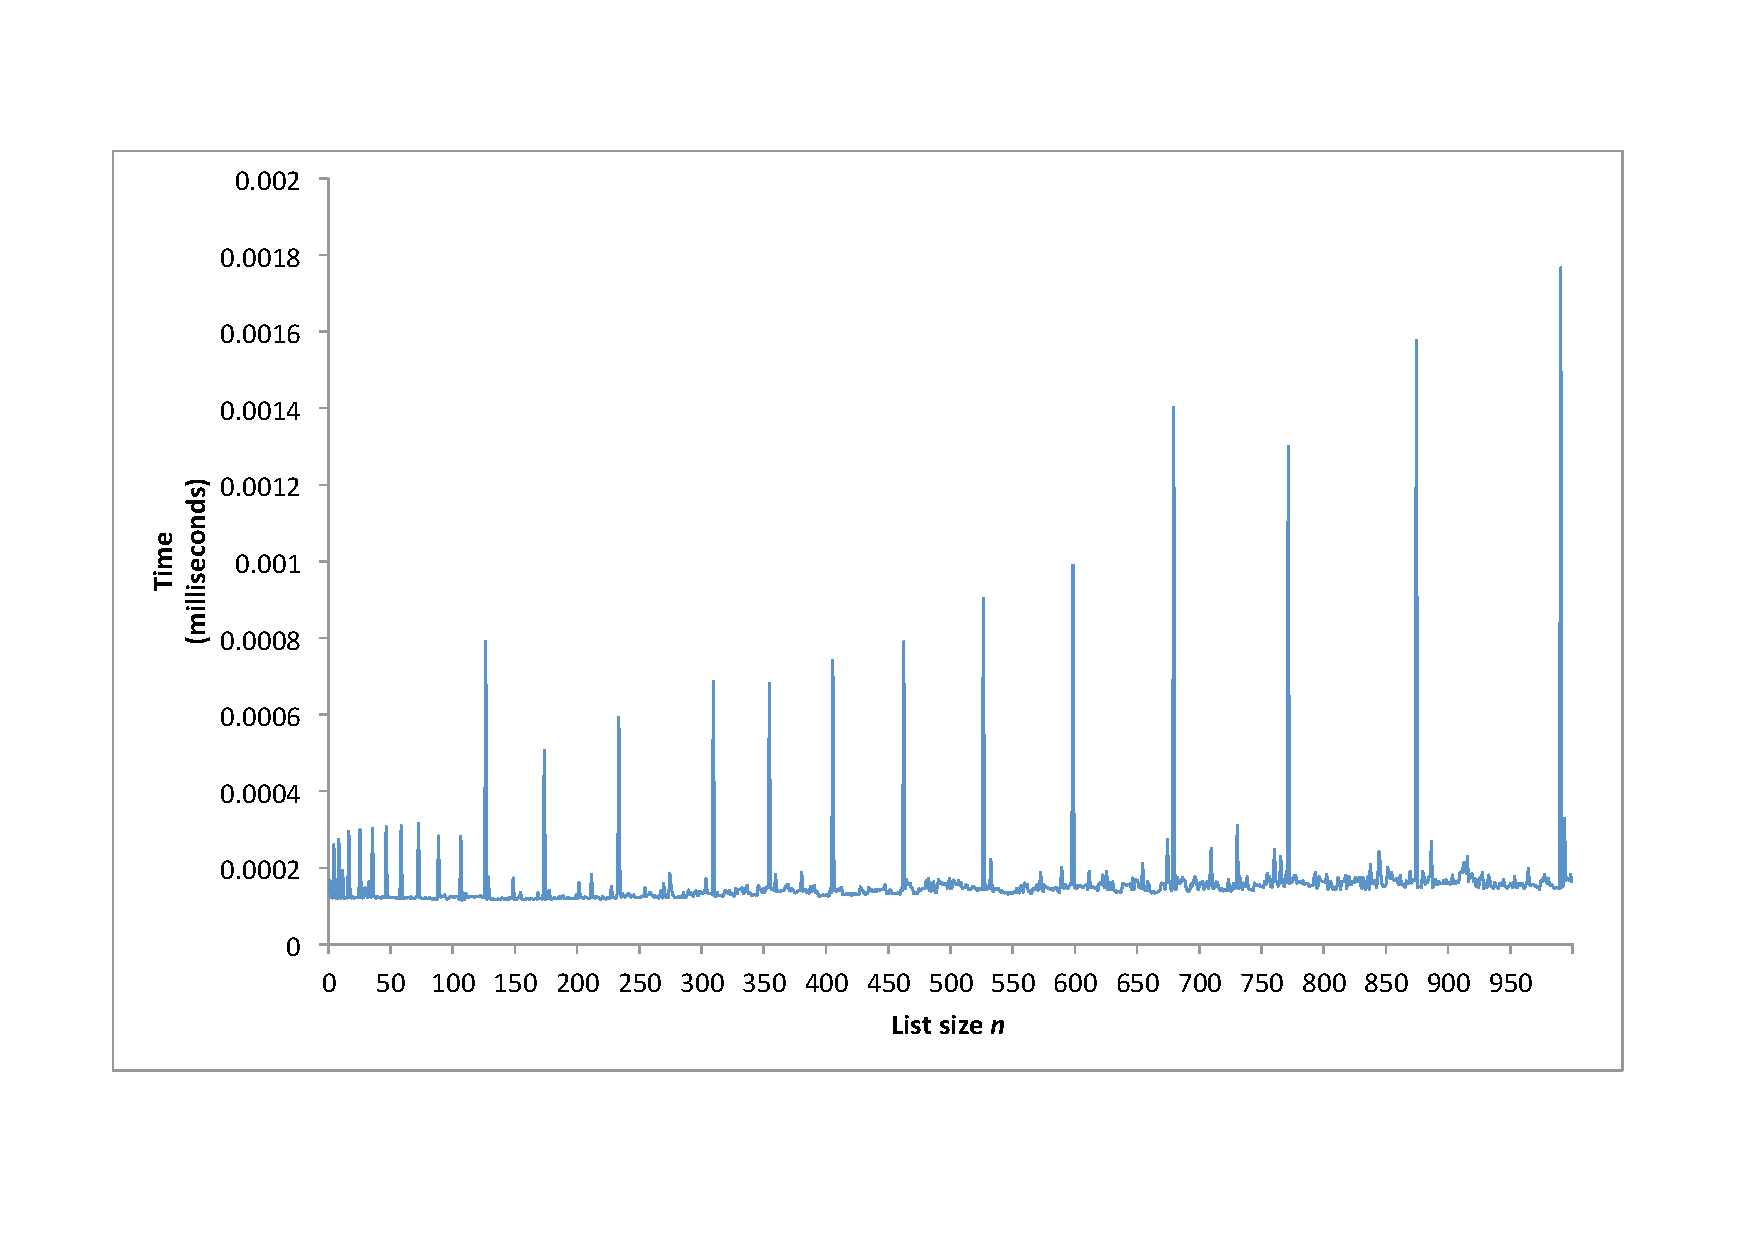
\includegraphics[height=0.9\textheight]{list_append_timing}
	\end{center}
\end{frame}

\begin{frame}{Operations on lists}
	\begin{itemize}
		\pause\item \textbf{Appending} to a list is \textbf{amortised constant time}
			\begin{itemize}
				\pause\item Usually $O(1)$, but can go up to $O(n)$ if the list needs to change size
			\end{itemize}
		\pause\item \textbf{Inserting} anywhere other than the end is \textbf{linear time}
			\begin{itemize}
				\pause\item Can't just insert new bytes into a memory block ---
					need to move all subsequent list elements to make room
			\end{itemize}
		\pause\item Similarly, \textbf{deleting} anything other than the last element is \textbf{linear time}
	\end{itemize}
\end{frame}

\begin{frame}{Tuples}
	\begin{itemize}
		\pause\item Tuples are like lists, but are \textbf{immutable}
			\begin{itemize}
				\pause\item Read-only
				\pause\item Once created, can't be changed
			\end{itemize}
		\pause\item Useful for storing sequences of values where adding, inserting, deleting or
			changing individual values does not make sense
			\begin{itemize}
				\pause\item E.g.\ $xy$ coordinates, RGB colours, ...
			\end{itemize}
		\pause\item Create tuples with \lstinline{()}, just as you create lists with \lstinline{[]}
			\begin{itemize}
				\pause\item Exception: a single element tuple is created as \lstinline{(foo,)}
					because \lstinline{(foo)} would be interpreted as a bracketed expression
			\end{itemize}
		\pause\item Can often omit the parentheses entirely, e.g.\ \lstinline{my_tuple = 1,2,3}
	\end{itemize}
\end{frame}

\begin{frame}[fragile]{Unpacking}
	If \lstinline{foo} is a list or tuple of length 4, the following are equivalent:
	\pause
	\begin{columns}
		\begin{column}{0.48\textwidth}
			\begin{lstlisting}
a, b, c, d = foo
			\end{lstlisting}
		\end{column}
		\pause
		\begin{column}{0.48\textwidth}
			\begin{lstlisting}
a = foo[0]
b = foo[1]
c = foo[2]
d = foo[3]
			\end{lstlisting}
		\end{column}
	\end{columns}
	\begin{itemize}
		\pause\item Unpacking requires the number of elements to match exactly ---
			if \lstinline{foo} has more than 4 elements, the code on the left will give an error
	\end{itemize}
\end{frame}

\begin{frame}[fragile]{One weird trick (Java programmers hate it!)}
	The following are equivalent:
	\pause
	\begin{columns}
		\begin{column}{0.48\textwidth}
			\begin{lstlisting}
a, b = b, a
			\end{lstlisting}
		\end{column}
		\pause
		\begin{column}{0.48\textwidth}
			\begin{lstlisting}
temp = a
a = b
b = temp
			\end{lstlisting}
		\end{column}
	\end{columns}
\end{frame}

\begin{frame}[fragile]{Strings are immutable}
	\begin{itemize}
		\pause\item \textbf{Strings} are immutable in Python
			\begin{itemize}
				\pause\item This is not true of all programming languages
			\end{itemize}
		\pause\item But wait... we change strings all the time, don't we?
	\end{itemize}
	\begin{lstlisting}
my_string = "Hello "
my_string += "world"
	\end{lstlisting}
	\begin{itemize}
		\pause\item This isn't changing the string, it's creating a new one and throwing the old one away!
		\pause\item Hence building a long string by appending can be slow (appending strings is $O(n)$)
	\end{itemize}
\end{frame}

\begin{frame}{Dictionaries}
	\begin{itemize}
		\pause\item Dictionaries are \textbf{associative maps}
		\pause\item A dictionary maps \textbf{keys} to \textbf{values}
			\begin{itemize}
				\pause\item Keys must be immutable (numbers, strings, tuples etc)
				\pause\item Values can be anything (including dictionaries or other containers)
			\end{itemize}
		\pause\item A dictionary is implemented as a \textbf{hash table}
	\end{itemize}		
\end{frame}

\begin{frame}[fragile]{Using dictionaries}
	\pause Create them using \lstinline|{}|:
	\begin{lstlisting}
age = {"Alice": 23, "Bob": 36, "Charlie": 27}
	\end{lstlisting}
	\pause Access values using \lstinline{[]}:
	\begin{lstlisting}
print(age["Alice"]) # prints 23
age["Bob"] = 40     # overwriting an existing item
age["Denise"] = 21  # adding a new item
	\end{lstlisting}
\end{frame}

\begin{frame}[fragile]{Iterating over dictionaries}
	\pause Iterating over a dictionary gives the \textbf{keys}:
	\begin{lstlisting}
for x in age:
    print(x)   # prints Alice, Bob, Charlie
	\end{lstlisting}
	\pause Use \lstinline{items} to get \textbf{key,value} pairs:
	\begin{lstlisting}
for key, value in age.items():
    print(key, "is", age, "years old")
	\end{lstlisting}
\end{frame}

\begin{frame}{Sets}
	\begin{itemize}
		\pause\item Sets are like dictionaries without the values
		\pause\item Sets are \textbf{unordered} collections of \textbf{unique} elements
            \begin{itemize}
                \pause\item Sets \textbf{cannot} contain \textbf{duplicate} elements
                \pause\item Attempting to \lstinline{add} an element already present in the set does nothing
            \end{itemize}
		\pause\item Certain operations on sets scale better on average than the equivalent operations on lists:
	\end{itemize}
	\pause
	\begin{center}
		\begin{tabular}{|c|c|c|}
			\hline
			\textbf{Operation} & \textbf{List} & \textbf{Set} \\\hline
			Add element & Append: $O(1)$ & $O(1)$ \\
			& Insert: $O(n)$ & \\\hline
			Delete element & $O(n)$ & $O(1)$ \\\hline
			Contains element? & $O(n)$ & $O(1)$ \\\hline
		\end{tabular}
	\end{center}
\end{frame}

\begin{frame}[fragile]{Using sets}
    \pause Create them using \lstinline|{}|:
	\begin{lstlisting}
numbers = {1, 4, 9, 16, 25}
	\end{lstlisting}
	\pause Add and remove members with \lstinline{add} and \lstinline{remove} methods
	\begin{lstlisting}
numbers.add(36)
numbers.remove(4)
	\end{lstlisting}
	\pause Test membership with \lstinline{in} operator
	\begin{lstlisting}
if 9 in numbers:
    print("Set contains 9")
	\end{lstlisting}
\end{frame}
